\clearpage
\section{Model description}
\label{sec:ModelDescr}

Natural Gas infrastructure, being a set of physically interconnected elements forming a network structure, can be represented with a graph. In mathematical term, a graph is an ordered pair $\mathcal{G} = (\mathcal{V}, \mathcal{E})$, where $\mathcal{V}$  is a set of elements called vertices (or nodes) and $\mathcal{E}$  an ordered set of vertex pairs called directed edges (or directed branch). Therefore, in a physical network representation, a directed edge represents any element of the network connecting an inlet and an outlet node with a defined direction. With such a schematization, the fluid-dynamic variables are associated to topological entities in this way:

\begin{itemize}
    \item nodal: pressure ($p$), exchanged mass flow rate with external environment ($\dot m_{ext}$, $G_{ext}$ or $L$), gas composition (molar fraction);
    \item branch: mass flow rate ($\dot m$ or $G$).
\end{itemize}

To be able to consider the variety of elements in a real gas network, nodes and branches shall be categorized in different types.
The following two paragraphs are devoted to the description of the possible types of \textit{nodal stations} and of \textit{branch elements}.
Subsections \ref{sec:ModelDescr_NodeSt} and \ref{sec:ModelDescr_BranchSt} are meant to describe the main implemented stations, items of the gas network which requires specifications such as set-points, operational limits etc. which acts like boundary conditions (with their profile in time if they are changing in time) and the technical parameters (such as diameters, length, heigh, etc.). When \textit{quality tracking and admixing} is to be performed, among the boundary conditions the specification of the nodal composition in the gas entry points acts as the boundary condition for the quality tracking problem.
The reader is then referred to the subsequent section (Sect.~\ref{sec:database}) where the database structure for data input/output is described. In this way, the structure of each table would be easily understood.

Subsection \ref{sec:NetwModRationale} briefly explains the fluid-dynamic solver part of the overall gas network model, which is also addressed more in-depth in Sect. \ref{sec: numerical_methods}. Overall, the model is summarized in the flow chart of Fig. \ref{modeldescr:flowchart}.
It is possible to note that, after the data acquisition and initialization phase, the time cycle starts. For each timestep, the gas quality is defined and an iterative procedure is followed to solve the linearized fluid-problem. Once a first solution is reached, the verification of the constraints posed on relevant nodal stations and branch element is performed. If one of these items displays a violation of the constraints, then the station state (e.g. control mode) is changed and the fluid-dynamic problem should be re-calculated from scratch, as some of the boundary conditions have been changed. 
When an acceptable solution is reached, the fluid network has been solved (i.e. all the nodal pressures, the pipeline mass flow rates and the nodal inward/outward mass flow rates have been determined). This result allows to address the quality tracking and admixing box: along the pipeline, the gas quality movement is tracked according to the velocities calculated from the step before, thus a spatial discretization is desired. At mixing nodes (i.e. when two pipelines converge in one node), the gas admixing is simulated, solving a mass balance equation for each chemical specie (the model can handle up to 21 chemical species, as the GERG-2008 equation of state is implemented).
When the quality box calculation have been terminated, the time counter is updated and a new time cycle is addressed, in which the gas quality is updated according to the result of the step before and the old solution of pressure and mass flow rate is used as representative of the previous time step.

The model have been consturcted such that it is possible to choose whether to perform an unsteady (transient) simulation or a seady-state one, with or without quality tracking.
In case of steady state with quality tracking, only the "admixing" procedure is possible: the result will then be representative of an equilibrium state, even from the point of view of the gas quality distribution.

\begin{figure}[H]
    \centering
    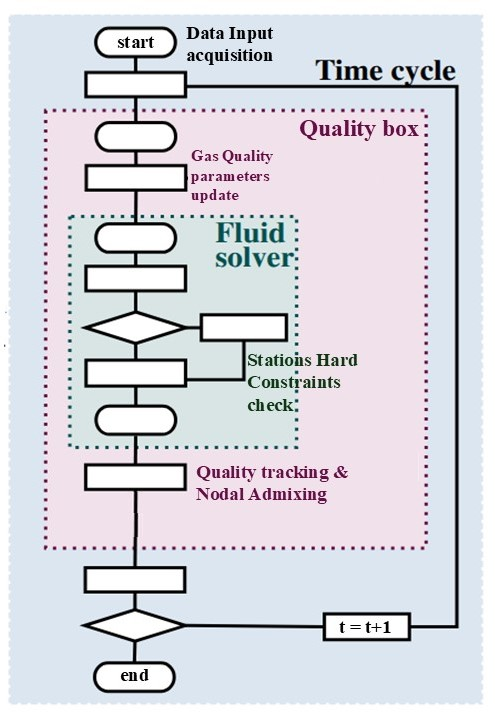
\includegraphics[scale = 0.6]{img_model descript/Shimmer++ flow chart basic.jpg}  
    \caption{Overall gas network model flow chart.}
    \label{modeldescr:flowchart}
\end{figure}

%%%%%%%%%%%%%%%%%%%%%%%%%%%%%%%%%%%%%%%%%%%%%%%%%%%%%%%%%%%%%%%%%%%%%%%%%%%%%%%%
\subsection{Nodal station types}
\label{sec:ModelDescr_NodeSt}
The nodes are generally the interfaces between the gas network and the outer world. For this reason, these are the elements on which to assign the boundary conditions. The quantities which can be assigned are, alternatively, the nodal pressure $p_n$ or the nodal mass flow rate $L_n$ exchanged with the external environment. The convention of the sign for the  nodal mass flow rate $L_n$ is as follows
\begin{itemize}
    \item exiting nodal mass flow rate (consumption) $\rightarrow$  $L_n > 0$
    \item entering nodal mass flow rate (injection) $\rightarrow$  $L_n < 0$.
\end{itemize}

Each node station is topologically and unambiguously defined by a node number $n$. Additionally, localization information can also be added such as: latitude and longitude coordinates and the altitude. While the first two information does not enter into the fluid-dynamic model (they might be useful for postprocessing of results) the altitude is in fact used to take into account the gravitational effect on the pressure drop calculation within the pipelines.

Given that, in general, the simulation is of an unsteady state, the boundary conditions may change over time either in value and in the controlled variable itself, defining the "state" of the nodal station. In the following, a list of the available nodal station, their control states and the related boundary conditions are given.
All the limits that, if surpassed, cause a switch in the control mode (thus a switch in state) are referred to as \textit{"Hard Limits"}.
\textit{"Soft Limits"} are instead intended to be the normal or desired working conditions. When they are surpassed, a warning message is given, but no further actions are automatically taken from the model.
%%%%%%%%%%%%%%%%%%%%%%%%%%%%%%%%%%%%%%%%%%%%%%%%%%%%%%%%%%%%%%%%%%%%%%%%%%%%%%%%
\subsubsection{Pressure regulated entry station without backflow}
Pressure regulated entry points can be associated with city-gate gas entry points or with llower-levelgas reduction stations as well as the gas entry point of a transmission system. In all these cases, these items are devoted to maintaining a fixed pressure setpoint at the relevant node. When dealing with the modelling of old types of reduction stations, the pressure set-point is fixed and constant throughout the whole simulation period. If a modulating-pressure reduction station is to be modelled, then the pressure boundary condition will be a time series of predefined pressure set-points. 
When providing a pressure set point to a node of the network, the gas flow rate  will be calculated as a consequence of the fluid-dynamic of the network in order to respect the constraint set by the boundary condition. 

This pressure regulated station is also referred to as ReMi station w/o backflow (ReMi is the Italian acronym for the Regulation and Metering stations, usually at the distribution network entry gates).
They are usually controlled in pressure, but their architecture is such that in case of any overpressure in the downstream portion of the network (meaning that the pressure on the distribution system side is higher than the pressure set-point), the gas flux is stopped. 

This pressure regulated station has as internal hard limit the following condition
\begin{equation}
L_n(t) \le 0.
\end{equation}
If it is not respected, then the control mode switches from pressure based to gas flow based and becomes
\begin{equation}
L_n(t) = 0,
\end{equation}
so to forbid any reverse gas flow. 
Through these set of boundary condition a typical Re-Mi gas station or second level gas reduction station is modelled: these items in fact are meant to reduce pressure from higher pressure level to distribution range ones, by setting an outlet pressure set point. Nevertheless, this kind of station can also be used for transmission system applications, whenever a pressure regulated control entry point is needed.
In Fig. \ref{model_description:architecture}, the graphical flowchart is given to explain the switch of states.

\begin{figure}[h]
    \centering
    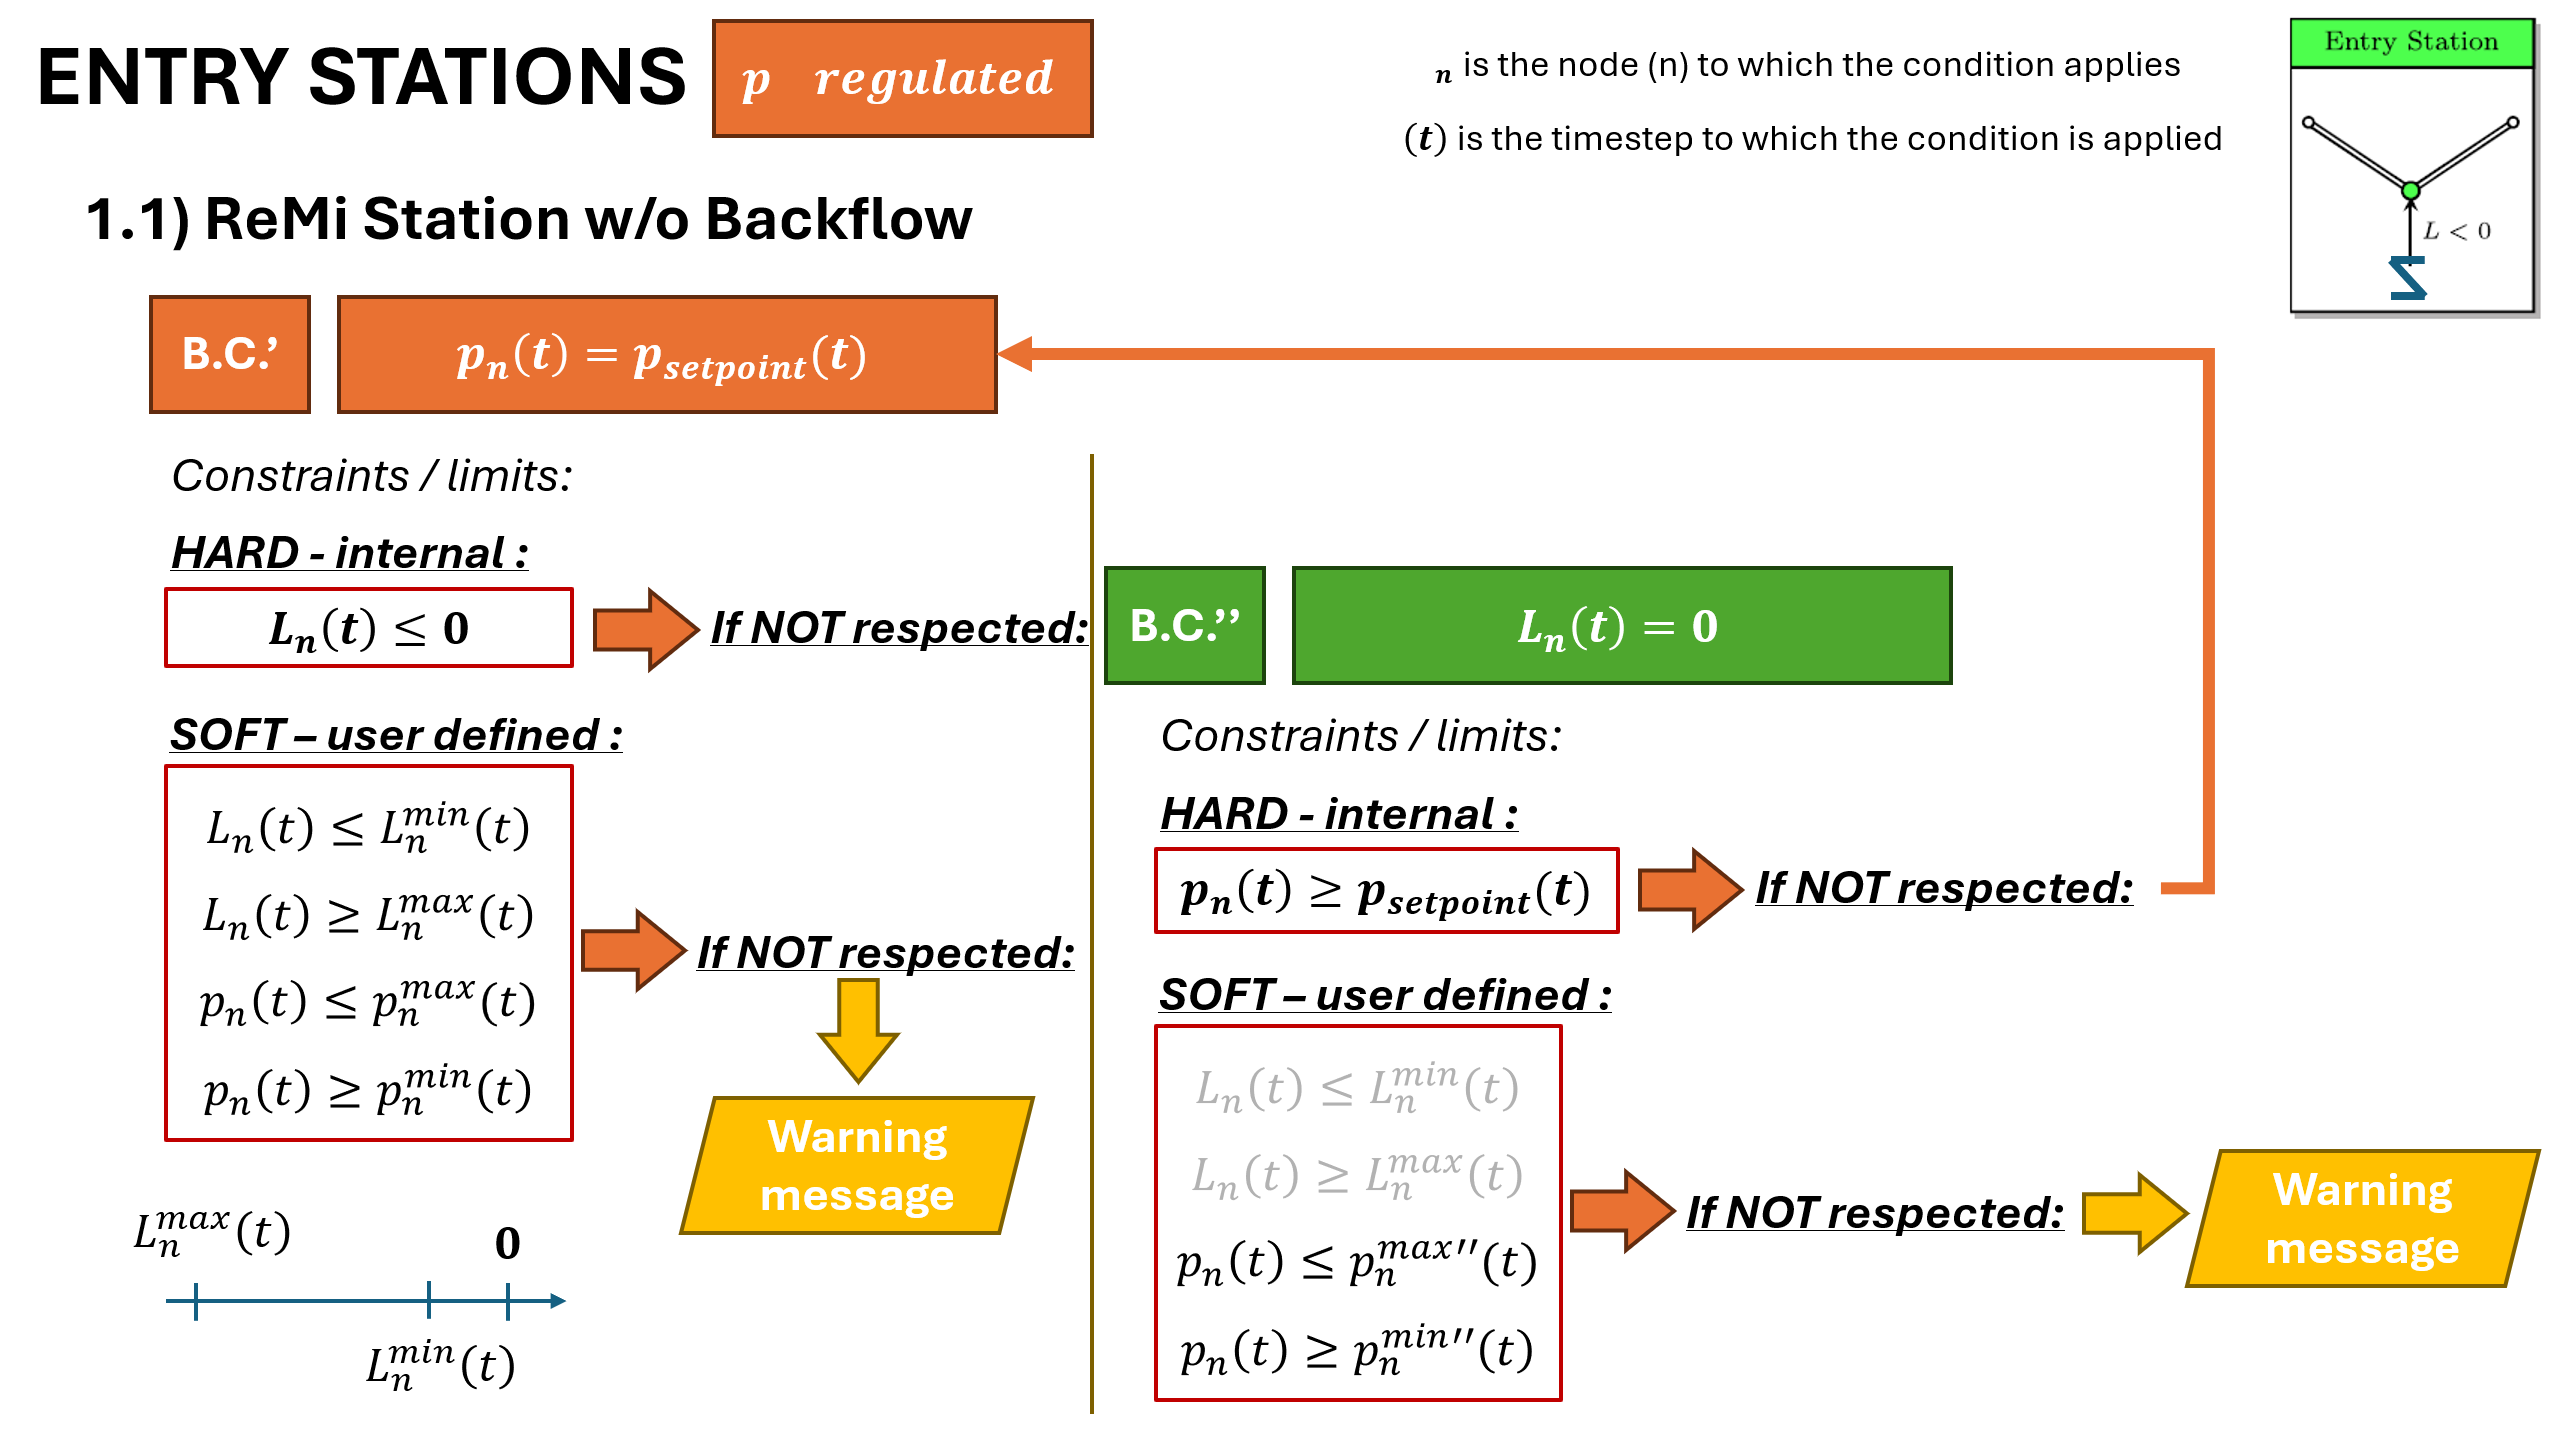
\includegraphics[scale = 0.22]{img_model descript/Entry Station P Regulated}  
    \caption{Pressure regulated entry station w/o backflow - flowchart representation.}
    \label{model_description:architecture}
\end{figure}

%%%%%%%%%%%%%%%%%%%%%%%%%%%%%%%%%%%%%%%%%%%%%%%%%%%%%%%%%%%%%%%%%%%%%%%%%%%%%%%%
\subsubsection{Mass Flow regulated entry station with pressure control}
Flow rate regulated entry points can be associated with gas entry points of the network where a known flux must be delivered: these are, for example, gas production fields, biomethane plants and, in perspective, hydrogen production and injection points (for blending purposes).
When providing a flow rate set point to a node of the network, the nodal pressure will be calculated as a consequence of the fluid-dynamic of the network calculated in order to respect the constraint set by the boundary condition. 

This mass flow regulated station has as internal hard limit the following condition:
\begin{equation*}
p_n(t) \le p_{\text{threshold}}(t) = f \cdot p_{\text{setpoint}}(t),
\end{equation*}
with the parameter $f \in [0, 1]$ representing a \textit{relative threshold factor} with respect to the setpoint value. 
It defines the maximum admissible fraction of the setpoint that the variable \( p_n(t) \) can reach. When \( p_n(t) \) exceeds \( f \cdot p_{\text{setpoint}}(t) \), the control mode switches from gas flow based to pressure control and becomes:
\begin{equation*}
p_n(t) \le p_{\text{setpoint}}(t).
\end{equation*}

Given a certain gas flow rate forced to enter the gas network, if the reached pressure in the injection point is higher than a certain pressure threshold, it might not be possible for the station or acceptable for the network to receive and then, a pressure set point should be put in force to calculate the allowable entering gas flux. This simulates cases of curtailments of renewable gases from the gas network. 

In Fig. \ref{model_description:architecture}, the graphical flowchart is given to explain the switch of states.

\begin{figure}[H]
    \centering
    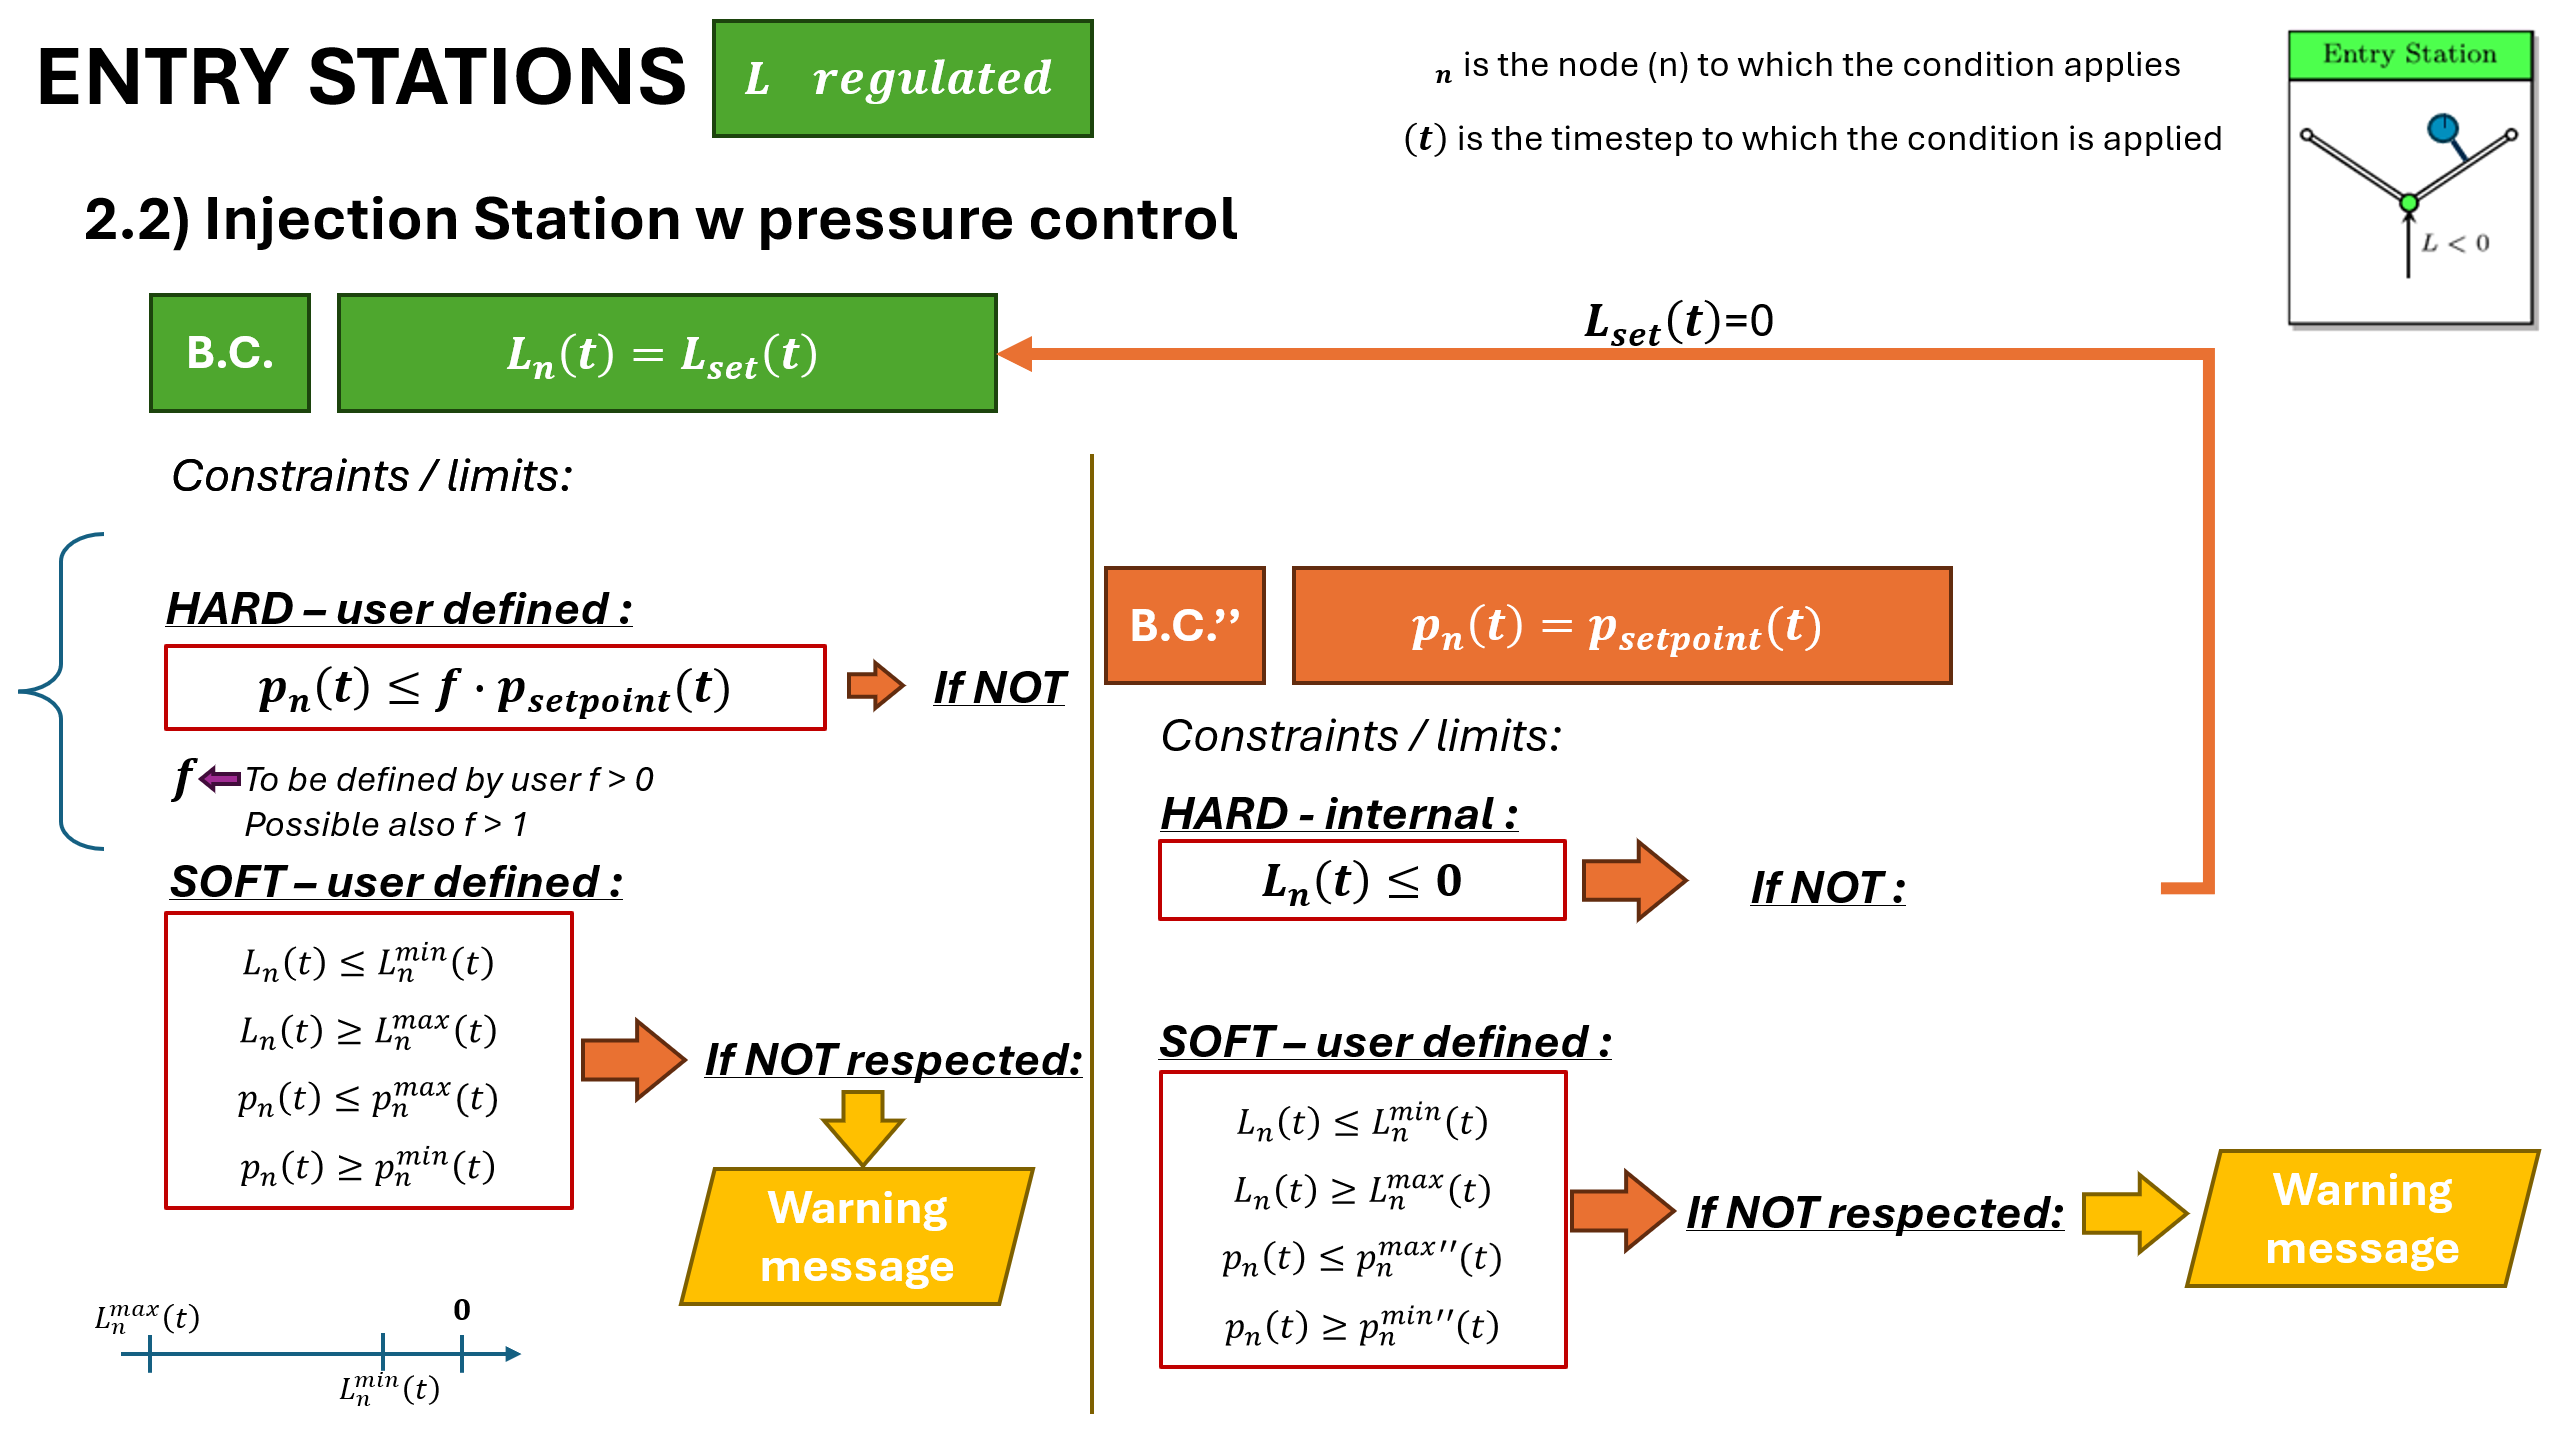
\includegraphics[scale = 0.22]{img_model descript/Entry Station L Regulated}  
    \caption{Mass regulated entry station w pressure control - flowchart representation.}
    \label{model_description:architecture}
\end{figure}
%%%%%%%%%%%%%%%%%%%%%%%%%%%%%%%%%%%%%%%%%%%%%%%%%%%%%%%%%%%%%%%%%%%%%%%%%%%%%%%%
\subsubsection{Junctions}
These are nodes that does not interacts with the external environment: they do not exchange any mass flow.
From a boundary condition point of view:
\begin{equation*}
L_n(t) = 0 \qquad \text{for any time } t
\end{equation*}
Consequently, the nodal pressure  \( p_n(t) \) is computed for any timestep.
It is to be highlighted that, in the Shimmer++ architecture, once a node is defined as \textit{"junction"}, this boundary conditions are automatically set.
%%%%%%%%%%%%%%%%%%%%%%%%%%%%%%%%%%%%%%%%%%%%%%%%%%%%%%%%%%%%%%%%%%%%%%%%%%%%%%%
\subsubsection{Exit Stations (consumption points)}
These nodes are the ones in which a consumption of gas is given. They can be seen as flow rate regulated stations without any control on the resulting pressure.
The user should here specify, for each timestep, the set value of consumption, providing the model with the gas consumption profile, with $L_n(t) \ge 0$. 


%%%%%%%%%%%%%%%%%%%%%%%%%%%%%%%%%%%%%%%%%%%%%%%%%%%%%%%%%%%%%%%%%%%%%%%%%%%%%%%%
%%%%%%%%%%%%%%%%%%%%%%%%%%%%%%%%%%%%%%%%%%%%%%%%%%%%%%%%%%%%%%%%%%%%%%%%%%%%%%%%

\subsection{Branch element types}
\label{sec:ModelDescr_BranchSt}

The branches are generally the connections between two nodes (either \textit{stations} or \textit{junctions}). Most of the time, they correspond to pipelines as physical entities. However, in the gas network infrastructure, at least two other physical entities can be modeled as branches: compression stations and pressure reduction stations. Basically, the first one is used to increase the pressure, and the second one is used to reduce the pressure.
Each branch-like element is topologically defined by 
\begin{itemize}
    \item inlet node $\rightarrow$  $n$ that should be consistent with the overall node numbering
    \item outlet node $\rightarrow$  $n$ that should be consistent with the overall node numbering
\end{itemize}

\subsubsection{Compression Station}

In this modeling framework, the compression station is considered as a black box that contains the combination of all the installed compressors and the gas coolers. In this way, the outlet gas temperature can be assumed the same as the one assumed throughout the system. The general form of the gas compressor equation referred to the mechanical shaft power $(P_{\text{shaft}})$ required by the compressor to the gas turbine driver, results in:
\[
P_{\text{shaft}} = \frac{1}{\eta_{is} \, \eta_{mecc}} 
   \frac{\gamma}{\gamma - 1} 
   Z_{in} \, T_{in} \, R_{in} 
   \left( \beta^{\frac{\gamma - 1}{\gamma}} - 1 \right) 
   \dot{m}_j
\]
with $\eta_{\text{is}}$  the isentropic efficiency of compression, $\eta_{\text{mecc}}$ the mechanical efficiency of the compressor (set equal to 80\%), $\gamma$ the adiabatic exponent, and $\beta$ the compression ratio which is the ratio between outlet and inlet pressure. $Z$, $T$, $R$ are respectively the gas compressibility factor, the temperature and the specific gas constant.

Similar to the nodal stations, the compression station needs the specification of a boundary condition that depends on its control mode. The compression station possible control modes are listed in Tab. \ref{tab:compressor:controls}
\begin{table}[h]
    \centering
    \begin{tabular}{ccc}
    \hline
    Controlled variable & Set point & Equation
    \\ \hline    
    Driver Power &  $P_{\text{shaft setpoint}}$ & $
P_{\text{shaft setpoint}} = \frac{1}{\eta_{is} \, \eta_{mecc}} 
   \frac{\gamma}{\gamma - 1} 
   Z_{in} \, T_{in} \, R_{in} 
   \left( \beta^{\frac{\gamma - 1}{\gamma}} - 1 \right) 
   \dot{m}_j
$ \\
    Outlet pressure  &  $p_{\text{outlet setpoint}}$ & $p_o = p_\text{o,setpoint}$\\
    Inlet pressure  &  $p_{\text{inlet setpoint}}$ & $p_i = p_\text{i,setpoint}$\\
    Pressure Ratio  &  $\beta_{\text{setpoint}}$ & $\frac{p_o}{p_i}=\beta_{\text{setpoint}}$\\
    Mass flow  &  $\dot{m}_{\text{setpoint}}$ & $\dot m_j = \dot m_\text{set}$\\
    \hline
    \end{tabular}
    \caption{Control modes for compressors.}
    \label{tab:compressor:controls}
\end{table}

The choice of one of this control mode changes the equation that simulate the compression station branch. 
Similar to the nodal stations, also for the compression stations some operative ranges of pressure, mass flow, pressure ratio and driver power should be specified as limits and, if violated, they may lead to changes in the control mode.

Furthermore, the gas compression station can also assume two different states: ON and OFF:
when the compressor is ON, one of the above-mentioned control mode needs to be specified;
when the compressor is OFF, two sub-states are possible (and should be specified):
\begin{itemize}
    \item BYPASS $\rightarrow$  $\dot{m}_{\text{in}}=\dot{m}_{\text{out}}$;  
    The compressor leaves free-flow thus the inlet and outlet mass (as well as the pressures) are set as equal.
    \item CLOSED $\rightarrow$  $\dot{m}_{\text{j,compr}}=0$
    The compressor acts like a closed valve. It interrupts the gas flow. This is relevant when the downstream section of the grid is at higher pressure than the upstream (so to avoid counterflows). 
\end{itemize}

%%%%%%%%%%%%%%%%%%%%%%%%%%%%%%%%%%%%%%%%%%%%%%%%%%%%%%%%%%%%%%%%%%%%%%%%%%%%%%%%
\begin{comment}
    
\subsubsection{Pressure Reduction Stations} 
\textcolor{red}{TO ALL --> IS IT IMPLEMENTED? WHAT TO DO?}
In this modeling framework, the Pressure Reduction Station is considered as a black box that contains the combination of all the installed items within a reduction stations (reduction valve, preheatiers etc). In this way, the outlet gas temperature can be assumed the same as the one assumed throughout the system. Being the pressure reduction stations passive elements of the network, their possible control modes are fewer than the ones of compression stations. For the sake of simplicity, in this modeling framework, the following has been considered
\begin{itemize}
    \item Outlet pressure control $\rightarrow$  $p_{\text{outlet setpoint}}$

    where $p_{\text{outlet setpoint}} \le p_{\text{inlet calc}} $
\end{itemize}
Furthermore, the pressure reduction station can also assume two different states: ON and OFF. 
When the station is ON, the above-mentioned control mode needs to be specified (i.e. input required by the user to specify the set point);
when the compressor is OFF, two sub-states are possible (and should be specified)
\begin{itemize}
    \item BYPASS $\rightarrow$  $\dot{m}_{\text{in}}=\dot{m}_{\text{out}}$
    
    The regulation station operates under free-flow conditions, thus the inlet and outlet mass (as well as the pressures) are set to be equal.
    \item CLOSED $\rightarrow$  $\dot{m}_{\text{compr}}=0$
   
    The  regulation station acts like a closed valve. It interrupts the gas flow. 
\end{itemize}

\end{comment}

%%%%%%%%%%%%%%%%%%%%%%%%%%%%%%%%%%%%%%%%%%%%%%%%%%%%%%%%%%%%%%%%%%%%%%%%%%%%%%%%
\subsubsection{Pipelines}

The pipelines are the most common branch-like items. They are fully passive elements with no boundary conditions requirements. Hence, each single pipe is defined by their technical parameters features, listed hereafter
\begin{itemize}
    \item Internal Diameter $\rightarrow$  $D_i$
    \item Length $\rightarrow$  $l$
    \item Internal Roughness $\rightarrow$  $\varepsilon_i$
\end{itemize}
In this modelling framework, in principle, the user can define pipelines with any lengths, which can differ a lot one-another. In case the user wants or need to have more uniform spatial discretization, it is possible to define the number of segments ($\#_{\text{segs}}$), for each node. The model will the subdivide the pipeline in the assigned number of segments, dividing uniformly the pipe length by creating a number of so-called "fictitius" nodes, treated as junctions.

The pipeline equation employed in this model is the Ferguson Equation, written as follows
\begin{equation*}
P_{in} - P_{out} e^{s_j}
= \frac{2 \, \bar{p}_j \, l_{e_j}}{A_j} \frac{\partial \dot{m}_j}{\partial t}
+ \frac{\lambda_j \, \bar{c}_j^{2} \, l_{e_j}}{D_j A_j^{2}} \, \dot{m}_j \lvert \dot{m}_j \rvert,
\end{equation*}
with
\[
l_{e_j} =
\begin{cases}
l_j, & h_{in} = h_{out} \\[8pt]
\dfrac{e^{s_j} - 1}{s_j} \, l_j, & h_{in} \neq h_{out}
\end{cases}
\qquad \text{ with  }
s_j = \dfrac{2 g (h_{out} - h_{in})}{\bar{c}_j^2},
\]
where $P=p^2$ is the quadratic pressure ($p$ in $[Pa]$), $\dot{m}_j$ is the gas mass flow rate $[kg/s]$, $\lambda$ is the friction factor $[-]$, $\bar{c}^{2}$ is the isothermal speed of sound of the gas $[m/s]$, $D_j$ is the pipeline inner diameter $[m]$, $A_j$ is the pipeline cross section area $[m^2]$, $l_j$ is the pipeline (or pipeline section) length $[m]$, $g$ is the gravitational acceleration $[m/s^2]$ and the subscripts \textit{in} and \textit{out} stand for the inlet and the outlet sections of the generic $j^{th}$ pipe. 
In order to account for the gravitational contribution, the ``effective length'' $l_e$ is defined as the corrected length of the pipeline section in case of non-horizontal pipelines (whose slope is defined by the elevation difference $(h_{out} - h_{in})$ of their ends).
The averaged quantities, which make the analytical solution possible,  are calculated starting from the computed value of the average pressure $\bar{p}$ as
\[
\bar{p} = \frac{p_{in}^2 + p_{in}p_{out} + p_{out}^2}{p_{in} + p_{out}},
\]
and in turn, the speed of sound is computed using the gas relation
\[
\bar{c}^2 = Z(\bar{p}, T, [y]) \, R T
\]
where $Z(\bar{p}, T, [y])$ is obtained from the application of the chosen gas Equation of State (EoS). In this modelling framework the GERG-2008 EoS has been implemented \cite{GERG}. Also the friction factor $\lambda$ can be calculated by means of an appropriate friction factor correlation. In this framework, the Cheng correlation is used \cite{CHENG}.

For an in-depth knowledge of the linearization and space-time discretization of the Ferguson formula the reader is invited to refer to \cite{Cavana2020} \cite{GREENSTREAM}.

%%%%%%%%%%%%%%%%%%%%%%%%%%%%%%%%%%%%%%%%%%%%%%%%%%%%%%%%%%%%%%%%%%%%%%%%%%%%%%%%

\subsection{Overall Network Model Rationale}
\label{sec:NetwModRationale}


Solving a fluid networks means to solve a pressure-velocity coupled problem on a graph-modeled infrastructure. 
In this case, the velocity variable has been replaced by the pipeline mass gas flow rates $\dot{m}_j$. For solving the gas network, two sets of equations are needed: a set of equations for all the branches and a set of equations for all the nodes. 
In this framework, the branch equations are the set of quadratic pressure drop equation which can be written for all the pipes (Fergusson Equation) and the nodal equations are the set of mass balance (mass conservation law) which can be applied to each nodes. Whenever a non-pipeline station is defined, the pressure drop equation is substituted with the relevant equation describing the element (and its control mode). Besides these, all the relevant boundary conditions are needed, as discribed in the previous sections.
By linearizing the pressure drop equation it is possible to assemble an algebraic problem for the full gas network infrastructure, provided that the topological structure of the network (i.e. all the node-branch connections) is properly arranged in an incidence matrix. To have more in-depth insight of this subject the reader is referred to \cite{GREENSTREAM}. In \ref{fig: scheme_model} a schematic representation of the mathematical procedure is displayed.

%%%%%%%%%%%%%%%%%%%%%%%%%%%%%%%%%%%%%%%%%%%%%%%%%%%%%%%%%%%%%%%%%%%%%%%%%%%%%%%%

\subsection{Nomenclature and unit of measurments}
\label{sec:NomAndUDM}

In this section, a summary table showing the units of measurement for each variable is given below:

\begin{table}[h!]
\centering
\renewcommand{\arraystretch}{1.25}
\setlength{\tabcolsep}{6pt}
\begin{tabular}{|>{\centering\arraybackslash}m{2.2cm}|
                >{\raggedright\arraybackslash}m{5.2cm}|
                >{\centering\arraybackslash}m{3.6cm}|
                >{\centering\arraybackslash}m{3.2cm}|}
\hline
\multicolumn{1}{|c|}{} &
\textbf{Input/output variable} &
\textbf{Symbol} &
\textbf{Unit of measurement} \\
\hline
\multirow{5}{*}{\rotatebox{90}{\textbf{Nodal variables}}}
 & Pressure & $p$ & Pa \\ \cline{2-4}
 & Injected/consumed gas & $\dot m_{\text{ext}}$ or $G_{\text{ext}}$ or $L$ & kg/s \\ \cline{3-4}
 &  & \textit{Injected} & \textit{negative value} \\ \cline{3-4}
 &  & \textit{Consumed} & \textit{positive value} \\ \cline{2-4}
 & Gas composition & \texttt{Frac\_XX} & Molar fraction [0--1] \\
\hline
\multirow{10}{*}{\rotatebox{90}{\textbf{Branch variables}}}
 & Mass flow & $\dot m$ or $G$ & kg/s \\ \cline{3-4}
 &  & \textit{Same direction of the branch} & \textit{Positive value} \\ \cline{3-4}
 &  & \textit{Opposite direction of the branch} & \textit{Negative value} \\ \cline{2-4}
 & Velocity & $v$ & m/s \\ \cline{3-4}
 &  & \textit{Same direction of the branch} & \textit{Positive value} \\ \cline{3-4}
 &  & \textit{Opposite direction of the branch} & \textit{Negative value} \\ \cline{2-4}
 & Diameter & $D$ & m \\ \cline{2-4}
 & Length & $l$ & m \\ \cline{2-4}
 & Roughness & $\varepsilon$ & m \\ \cline{2-4}
 & Compressor power & $P_{\text{cmpr}}$ & W \\
\hline
\end{tabular}
\caption{Nodal and branch variables with their symbols and units of measurement.}
\label{tab:variables}
\end{table}





%%%%%%%%%%%%%%%%%%%%%%%%%%%%%%%%%%%%%%%%%%%%%%%%%%%%%%%%%%%%%%%%%%%%%%%%%%%%%%%%

%%%%%%%%%%%%%%%%%%%%%%%%%%%%%%%%%%%%%%%%%%%%%%%%%%%%%%%%%%%%%%%%%%%%%%%%%%%%%%%%
%%%%%%%%%%%%%%%%%%%%%%%%%%%%%%%%%%%%%%%%%%%%%%%%%%%%%%%%%%%%%%%%%%%%%%%%%%%%%%%%